\chapter{Quintor}
\textit{In dit hoofdstuk zal er inzicht gegeven worden over het bedrijf Quintor waar het afstudeerproject heeft plaatsgevonden. Er wordt verteld over de diensten die Quintor levert en wat de doelen zijn van de organisatie. Er zal ook kort toegelicht worden waar de afstudeerder binnen het bedrijf opereert en welke werknemers vanuit Quintor betrokken zijn bij de afstudeeropdracht.
}

Quintor is een toonaangevend bedrijf op het gebied van Agile software development, Enterprise Java / .NET technologie en mobile development. Het bedrijf is begonnen in 2005 in Groningen en is opgericht door Johan Tillema, de huidige CEO van het bedrijf. Sinds 2005 heeft het bedrijf een gezonde groei doorgemaakt en heeft inmiddels 150 medewerkers, verspreid over vestigingen in Groningen, Amersfoort en Den Haag. Vanuit deze vestigingen ondersteunt het bedrijf klanten bij de uitdagingen die grootschalige Enterprise projecten met zich meebrengen. Het succes van Quintor is te danken aan drie pijlers: techniek en architectuur, een hoogwaardige ontwikkelstraat en het Agile/Scrum proces. Tevens beschikt Quintor over een Software Factory waarin in-house projecten voor klanten worden uitgevoerd.

\section{Software Factory}

In de Software Factory staat alle kennis en expertise die Quintor heeft verzameld over de jaren heen. Het is een hoogwaardig platform waarin de tooling, standaarden en best practices en tevens een complete oplossing is voor het managen en hosten van Scrum projecten. Dit wordt onder andere gebruikt om klanten te helpen bij het professionaliseren en efficiënter inrichten van softwareontwikkeling. Een groot deel van de werkzaamheden die Quintor dan ook uitvoert voor klanten is consultatie bij o.a. het implementeren van Agile/Scrum werk- en denkwijze. Naast Java en .NET development behoort ook mobile development tot de kerncompetenties van Quintor, en is dan ook opgenomen in de Software Factory. Hieronder zijn een aantal onderdelen uitgelicht die voorkomen in de Software Factory.

\paragraph{Enterprise architectuur}

Vanuit een pragmatische insteek en op basis van jarenlange ervaring helpen de software architecten van Quintor organisaties bij het maken van de juiste keuzes op het gebied van architectuur. Hierbij gaat het om het zowel opstellen als implementeren van een architectuur.

\paragraph{Informatie analyse}

Het in kaart brengen van informatie door het gebruik van diverse analyse- en ontwerptechnieken zoals UML, user-stories en use-cases in een Agile omgeving.

\paragraph{Java en .NET development}

Het realiseren van duurzame IT-systemen, in-house of bij klanten, die naadloos aansluiten bij de wensen van de business. Hierbij zijn er een groot aantal van omvangrijke systemen ontwikkelt.

\paragraph{Agile/Scrum}

Agile/Scrum is een effectieve en flexibele methode die uitgaat van een iteratiefontwikkelproces. Het trainen van complete projectteams met een op maat gemaakte training, waarbij aansluitend support en coaching gegeven wordt.

\paragraph{Mobile development}

Mobiele applicaties voor iPhone, iPad en Android. Specifiek hiervoor is het 'Mobile development center' opgezet, waarin er apps ontworpen, ontwikkelt en beheert worden. Dit betreft de realisatie van stand-alone tot volledige geïntegreerde Enterprise apps.

\section{Visie}

Een van de doelstellingen die Quintor heeft is het professionaliseren van software development. Aansluitend daarop probeert het bedrijf continu voor te lopen op de concurrentie door het opdoen van kennis op het gebied van nieuwe technologieën, waarbij professionalisering van de werkwijze voorop staat.

\begin{formal}
  \label{visie}
  ``Onze ambitie: professionaliseren van software development."
  \\ Johan Tillema, Chief Executive Officer
\end{formal}

Door het aanbieden van uitdagende afstudeeropdrachten wordt er kennis opgebouwd die benodigd is om nieuwe technologieën, zoals bijvoorbeeld Machine Learning of Blockchain. Deze kennis kan ingezet worden om klanten te adviseren bij de uitdagingen die grootschalige Enterprise projecten met zich meebrengen en zal, middels het volwassen genoeg is, opgenomen worden in de Software Factory.

\section{Organisatie}
In fig. \ref{organogram} wordt de organisatie van Quintor weergegeven. Bovenaan staat Johan Tillema, de oprichter en CEO. Direct eronder staat het Secretariaat en het Recruitment Office. Hierin is te zien dat er vier segmenten zijn waarop er consultatie aangeboden wordt: development, analysis en design en front-end.

\begin{figure}[h]
  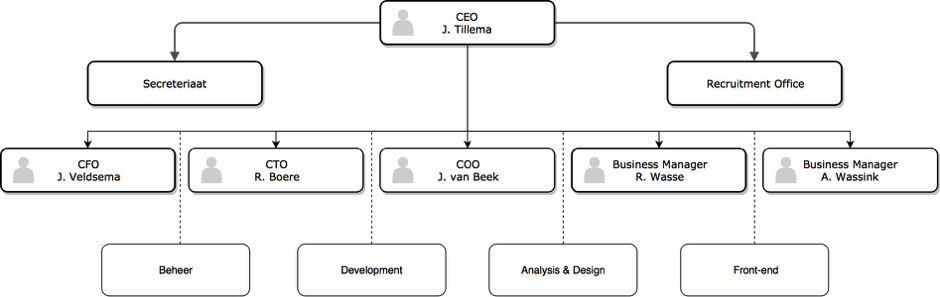
\includegraphics[width=1\textwidth]{figures/organogram}
  \caption{Organogram van Quintor.}
  \label{organogram}
\end{figure}

\newpage
Zelf val ik onder het development segment, waarbij er aangestuurd wordt door Ben Ooms, (beschreven in \ref{begeleider}). Er wordt zelfstandig gewerkt aan de opdracht waarbij er een aantal praktijken van Scrum toegepast zijn tijdens het afstudeertraject. Zo is er elke twee weken een zogenaamde demo dag waarbij iedere afstudeerder een demonstratie over waar hij of zij de afgelopen tijd mee bezig is geweest, en of er ergens tegenaan gelopen wordt zodat er samen nagedacht kan worden over mogelijke oplossingen.

\section{Betrokkenen}

Binnen Quintor zijn er een aantal medewerkers die nodig zijn om het project tot een geslaagd einde te brengen. Hieronder zijn deze medewerkers kort benoemd en wat hun rol is binnen het afstudeertraject.

\paragraph{Ben Ooms} \label{begeleider} is de begeleider van de afstudeeropdracht. Hij is een Java ontwikkelaar die als bijkomende taak heeft om de afstudeerders binnen Den Haag te begeleiden. Zijn uitvoerende taken hierbij zijn dan ook onder andere advies geven over de aanpak van de opdracht en waarbij mogelijk de voortgang van de opdracht te bevorderen.

\paragraph{Pim Otte} \label{expert} is de Blockchain expert binnen Quintor en heeft veelal ervaring met de toepassing en realisatie van applicaties die gebruik maken van Blockchain technologie. Hij is beschikbaar gedurende de afstudeeropdracht om inzichten en feedback te geven op de uitgevoerde werkzaamheden.

\paragraph{Kevin Bos} is afstudeerder afkomstig van Avans Hogeschool. Hij is verantwoordelijk voor het lokale gedeelte van de Blockchain opdracht. Tijdens de afstudeeropdracht is hij een stakeholder van het project en zal er een zekere mate van samenwerking aanwezig zijn.